\documentclass{beamer}
%SAND 2023-XXXX-O
\usepackage{comment}
\usepackage{color}
\usepackage{listings}
\usepackage{verbatim}
\usepackage{multicol}
\usepackage{booktabs}
\definecolor{green}{RGB}{0,128,0}

\def\EQ#1\EN{\begin{equation*}#1\end{equation*}}
\def\BA#1\EA{\begin{align*}#1\end{align*}}
\def\BS#1\ES{\begin{split*}#1\end{split*}}
\newcommand{\bc}{\begin{center}}
\newcommand{\ec}{\end{center}}
\newcommand{\eq}{\ =\ }
\newcommand{\degc}{$^\circ$C}

\def\p{\partial}
\def\qbs{\boldsymbol{q}}
\def\Dbs{\boldsymbol{D}}
\def\A{\mathcal A}
\def\gC{\mathcal C}
\def\gD{\mathcal D}
\def\gL{\mathcal L}
\def\M{\mathcal M}
\def\L{\mathcal L}
\def\P{\mathcal P}
\def\Q{\mathcal Q}
\def\gR{\mathcal R}
\def\gS{\mathcal S}
\def\X{\mathcal X}
\def\bnabla{\boldsymbol{\nabla}}
\def\bnu{\boldsymbol{\nu}}
\renewcommand{\a}{{\alpha}}
%\renewcommand{\a}{{}}
\newcommand{\s}{{\sigma}}
\newcommand{\bq}{\boldsymbol{q}}
\newcommand{\bz}{\boldsymbol{z}}
\def\bPsi{\boldsymbol{\Psi}}

\def\Li{\textit{L}}
\def\Fb{\textbf{f}}
\def\Jb{\textbf{J}}
\def\cb{\textbf{c}}

\def\Dt{\Delta t}
\def\tpdt{{t + \Delta t}}
\def\bpsi{\boldsymbol{\psi}}
\def\dbpsi{\delta \boldsymbol{\psi}}
\def\bc{\textbf{c}}
\def\dbc{\delta \textbf{c}}
\def\arrows{\rightleftharpoons}

\newcommand{\bGamma}{\boldsymbol{\Gamma}}
\newcommand{\bOmega}{\boldsymbol{\Omega}}
%\newcommand{\bPsi}{\boldsymbol{\Psi}}
%\newcommand{\bpsi}{\boldsymbol{\psi}}
\newcommand{\bO}{\boldsymbol{O}}
%\newcommand{\bnu}{\boldsymbol{\nu}}
\newcommand{\bdS}{\boldsymbol{dS}}
\newcommand{\bg}{\boldsymbol{g}}
\newcommand{\bk}{\boldsymbol{k}}
%\newcommand{\bq}{\boldsymbol{q}}
\newcommand{\br}{\boldsymbol{r}}
\newcommand{\bR}{\boldsymbol{R}}
\newcommand{\bS}{\boldsymbol{S}}
\newcommand{\bu}{\boldsymbol{u}}
\newcommand{\bv}{\boldsymbol{v}}
%\newcommand{\bz}{\boldsymbol{z}}
\newcommand{\pressure}{P}

\def\water{H$_2$O}
\def\calcium{Ca$^{2+}$}
\def\copper{Cu$^{2+}$}
\def\magnesium{Mg$^{2+}$}
\def\sodium{Na$^+$}
\def\potassium{K$^+$}
\def\uranium{UO$_2^{2+}$}
\def\hion{H$^+$}
\def\hydroxide{0H$^-$}
\def\bicarbonate{HCO$_3^-$}
\def\carbonate{CO$_3^{2-}$}
\def\cotwo{CO$_2$(aq)}
\def\chloride{Cl$^-$}
\def\fluoride{F$^-$}
\def\phosphoricacid{HPO$_4^{2-}$}
\def\nitrate{NO$_3^-$}
\def\sulfate{SO$_4^{2-}$}
\def\souotwooh{$>$SOUO$_2$OH}
\def\sohuotwocothree{$>$SOHUO$_2$CO$_3$}
\def\soh{$>$SOH}

\newcommand\gehcomment[1]{{{\color{orange} #1}}}
\newcommand\add[1]{{{\color{blue} #1}}}
\newcommand\remove[1]{\sout{{\color{red} #1}}}
\newcommand\codecomment[1]{{{\color{green} #1}}}
\newcommand\redcomment[1]{{{\color{red} #1}}}
\newcommand\bluecomment[1]{{{\color{blue} #1}}}
\newcommand\greencomment[1]{{{\color{green} #1}}}
\newcommand\magentacomment[1]{{{\color{magenta} #1}}}

\begin{comment}
\tiny
\scriptsize
\footnotesize
\small
\normalsize
\large
\Large
\LARGE
\huge
\Huge
\end{comment}

\begin{document}
\title{3D Four-Fracture Transport}
\author{Michael Nole and Rosie Leone}
\date{\today}

%\frame{\titlepage}


%-----------------------------------------------------------------------------
\section{Description of Four-Fracture Model}

\subsection{Four-Fracture Model}

\frame{\frametitle{Description of Four-Fracture Model Scenario}
The ``3D Four-Fracture Transport Model'' simulates solute transport through a fracture network using an equivalent continuous porous medium (ECPM) formulation. This multi-step problem includes the following:
\begin{itemize}
  \item Generating a four-fracture network using dfnWorks
  \item Upscaling the fracture network properties to an ECPM using mapdfn2pflotran.py
  \item Running a flow model on the fracture network in PFLOTRAN to steady state
  \item Restarting the model and running transport on the steady-state flow field in PFLOTRAN
  \item Visualizing results in ParaView
\end{itemize}

\bluecomment{Note: this practice problem requires dfnWorks to be installed. *This problem was last tested on dfnWorks commit aa02d61*}

}

\frame{\frametitle{Four-Fracture Scenario Conceptual Model}
	The ``3D Four-Fracture Transport Model'' simulates steady-state, fully-saturated groundwater flow through a network of four deterministic elliptical fractures upscaled to an equivalent continuous porous medium (ECPM). After establishing a steady-state flow field, a pulse of tracer is applied. The problem is parameterized as follows:
	
	\begin{itemize}
		\small
		\item Problem domain: $1000 \times 1000 \times 1000$ m (x $\times$ y $\times$ z)
		\item Grid resolution $20 \times 20 \times 20$ m
		\item Inflow (West) boundary pressure: 1.001 MPa
		\item Outflow (East) boundary pressure: 1 MPa
		\item Matrix properties
		\begin{itemize}
			\footnotesize
			\item Permeability: $1x10^{-18} m^{2}$
			\item Porosity: 0.005
			\item Tortuosity: 0.2
		\end{itemize}
	\end{itemize}

}

\frame{\frametitle{Four-Fracture Scenario Conceptual Model cont'd}
	\begin{itemize}
		\item Fracture properties
		\begin{itemize}
			\footnotesize
			\item Fracture 1
			\begin{itemize}
				\item Radius: 600 m
				\item Translation: [-400, 0, 200]
				\item Normal Vector: [30, 15, 60]
				\item Aperture: $\eq 1x10^{-3}$ m
			\end{itemize}
			\item Fracture 2
			\begin{itemize}
				\item Radius: 1000 m
				\item Translation: [0, 0, 0]
				\item Normal Vector: [95, 5, 0]
				\item Aperture: $\eq 1x10^{-3}$ m
			\end{itemize}
			\item Fracture 3
			\begin{itemize}
				\item Radius: 600 m
				\item Translation: [400, 0, 200]
				\item Normal Vector: [30, 15, 60]
				\item Aperture: $\eq 1x10^{-3}$ m
			\end{itemize}
			\item Fracture 4
			\begin{itemize}
				\item Radius: 600 m
				\item Translation: [-400, 0, 200]
				\item Normal Vector: [30, 15, 60]
				\item Aperture: $\eq 5x10^{-5}$ m
			\end{itemize}
		\end{itemize}
	\end{itemize}
	
}

%-----------------------------------------------------------------------------
\frame{\frametitle{Four-Fracture Scenario Schematic}
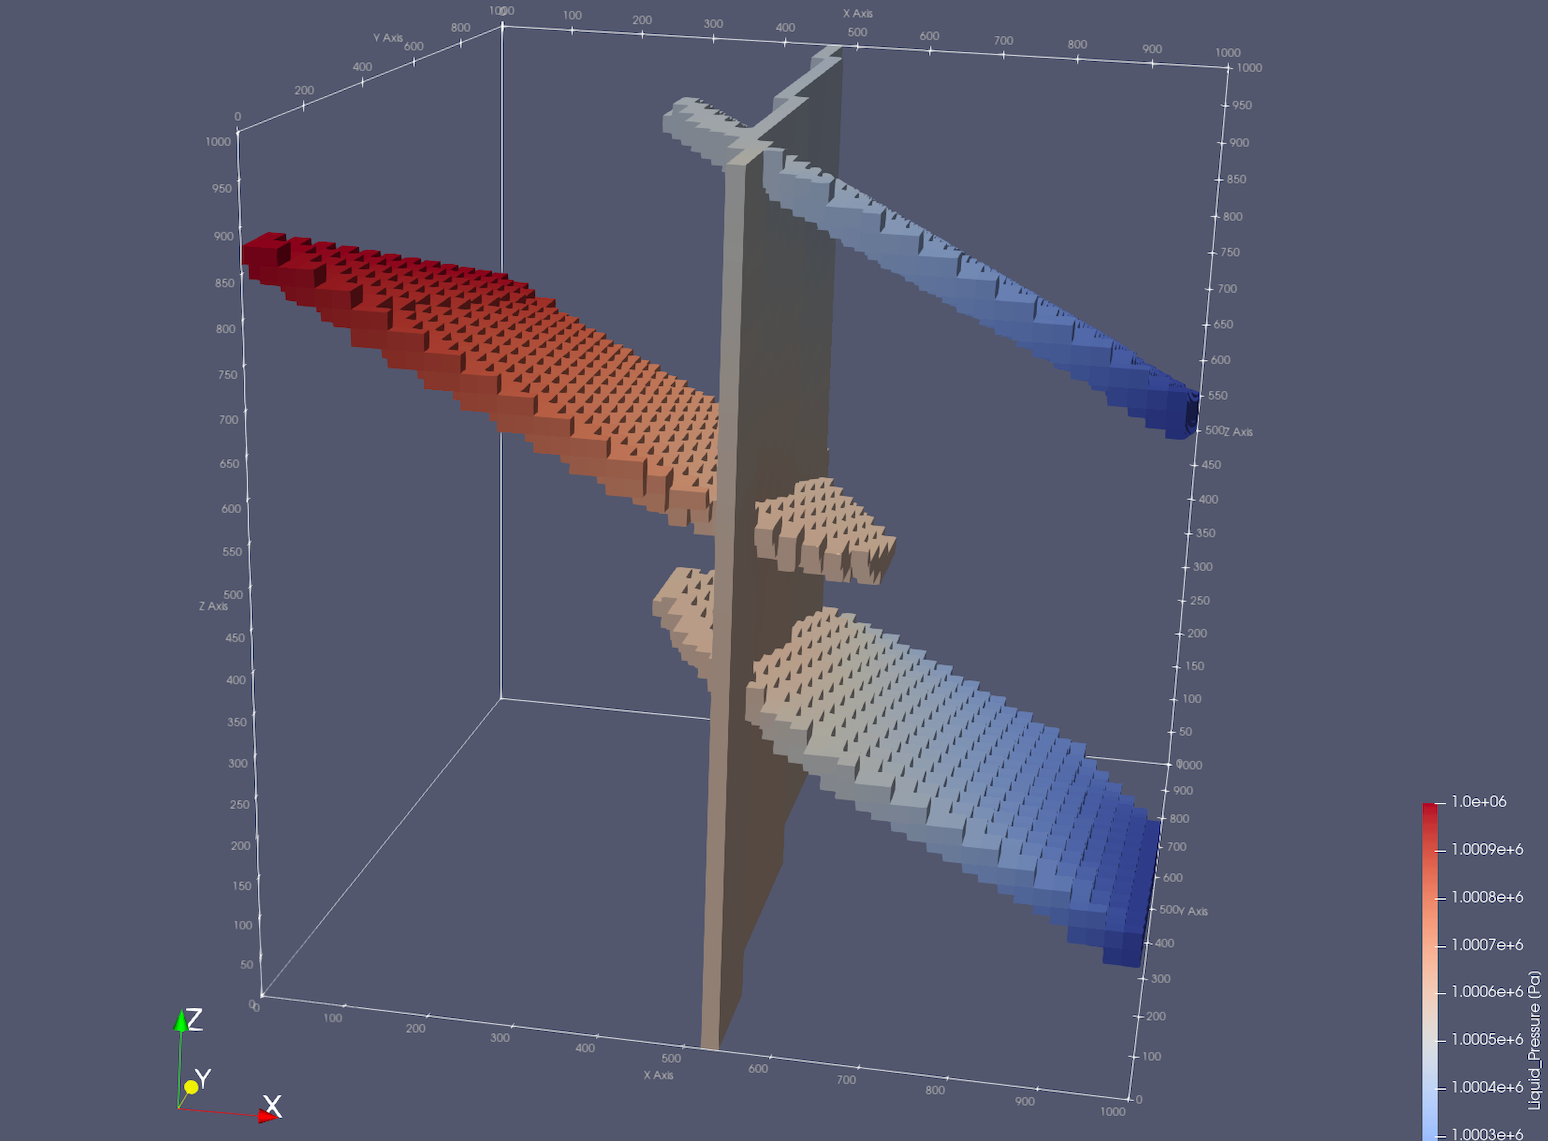
\includegraphics[width=\linewidth]{./4-frac}
}

%-----------------------------------------------------------------------------
\subsection{Governing Equations}
\frame{\frametitle{Governing Flow Equations: Richards Equation}
	
	{\bf Continuity Equation:}
	\EQ
	\frac{\p}{\p t} \big(\varphi s \rho\big) + \bnabla\cdot\rho\bq \eq Q
	\EN
	
	
	{\bf Darcy's Law:}
	\EQ
	\bq \eq -\frac{\bk k_r}{\mu} \bnabla\big(\pressure-\rho g z\big)
	\EN
	
	\normalsize
	
	\begin{columns}[c]
		\column{0.5\linewidth}
		\begin{itemize}
			\item $\varphi \eq $ porosity
			\item $s \eq $ saturation
			\item $\rho \eq $ water density
			\item $\bk \eq $ intrinsic permeability tensor
			\item $k_r \eq $ relative permeability
			\item $Q \eq $ source/sink
		\end{itemize}
		\column{0.5\linewidth}
		\begin{itemize}
			\item $\mu \eq $ viscosity
			\item $\pressure \eq $ water pressure
			\item $g \eq $ gravity
			\item $z \eq $ distance in direction of gravity
			\item $q \eq $ Darcy velocity
		\end{itemize}
	\end{columns}
	
	
}

\frame{\frametitle{Governing Reactive Transport Equations}
	
	\Large
	
	\EQ\label{trans}
	\frac{\p}{\p t} \left(\varphi s \Psi_j\right) + \bnabla\cdot\bOmega_j \eq
	\gR\left(c_1,c_2,\ldots,c_n\right)
	\EN
	
	\EQ\label{flux}
	\bOmega_j \eq \big(\bq - \varphi s \Dbs\bnabla\big) \Psi_j
	\EN
	
	%\bigskip
	%\normalsize
	\footnotesize
	\begin{align*}
		\varphi &\eq \text{porosity}; \quad
		s \eq \text{liquid saturation}\\
		\Psi_j &\eq \text{total component concentration for aqueous species } j\\
		c_j &\eq \text{free ion concentration for aqueous species } j\\
		\bOmega &\eq \text{solute flux}; \quad
		\bq \eq \text{Darcy velocity} \\
		\Dbs &\eq \text{hydrodynamic dispersion} \eq\gD^\ast + \alpha_L|\bnu|\\
		\gD^\ast &\eq \text{species-independent diffusion coefficient}\\
		\alpha_L &\eq \text{longitudinal dispersity}\\
		\bnu &\eq \text{pore water velocity} \eq \bq/\varphi
	\end{align*}
	
}

%-----------------------------------------------------------------------------
\section{Description of Inputs}

\subsection{DFN Generation}

\begin{frame}[fragile,containsverbatim]\frametitle{DFNWorks Inputs}
	
	\begin{itemize}
		\item \begin{semiverbatim}generateDFN.py :\end{semiverbatim}
		\item Import pydfnworks Python library. Then add fracture elements to the domain as follows:
	\end{itemize}
	
	\begin{semiverbatim}
		DFN = DFNWORKS(jobname)
		
		DFN.params['domainSize']['value'] =  \bluecomment{#domain size}
							[1000.0, 1000.0, 1000.0]
		
		DFN.params['h']['value'] = 5.0  \bluecomment{#discretization scale}
		
		DFN.add_user_fract(shape='ell', \bluecomment{#fracture shape}
			radii=600,                    \bluecomment{#fracture 1/2 size}
			translation=[-400, 0, 200],      \bluecomment{#fracture center}
			normal_vector=[30, 15, 60],      \bluecomment{#fracture plane normal}
			number_of_vertices=5,     \bluecomment{#points on fracture boundary}
			aperture=1.0e-3)      \bluecomment{#hydraulic aperature}   
			
	\end{semiverbatim}
	
\end{frame}

\begin{frame} [fragile,containsverbatim]\frametitle{DFNWorks Inputs cont'd}
		\begin{semiverbatim}
					
		DFN.add_user_fract(shape='ell',
		radii=1000,
		translation=[0, 0, 0],
		normal_vector=[95, 5, 0],
		number_of_vertices=5,
		aperture=1.0e-3)
		
		DFN.add_user_fract(shape='ell',
		radii=600,
		aspect_ratio=1,
		translation=[400, 0, 200],
		normal_vector=[30, 15, 60],
		number_of_vertices=5,
		aperture=1.0e-3)

	\end{semiverbatim}
\end{frame}

\begin{frame} [fragile,containsverbatim]\frametitle{DFNWorks Inputs cont'd}
	\begin{semiverbatim}
		
		DFN.add_user_fract(shape='ell',
		radii=600,
		aspect_ratio=1,
		translation=[400, 0, -400],
		normal_vector=[30, 15, 60],
		number_of_vertices=5,
		aperture=5.0e-5)
		
		DFN.make_working_directory(delete=True)
		DFN.print_domain_parameters()
		DFN.check_input()
		DFN.create_network()
		DFN.dump_hydraulic_values()
		
	\end{semiverbatim}
\end{frame}

\begin{frame} [fragile,containsverbatim]\frametitle{DFNWorks Outputs}
	From perm.dat:
	\begin{semiverbatim}
		8.333333333333332515e-08
		8.333333333333332515e-08
		8.333333333333332515e-08
		2.083333333333333377e-10
	\end{semiverbatim}
	From radii\_Final.dat:
	\begin{semiverbatim}
		Fracture Radii List After Isolated Fracture 
		   and Cluster Removal
		Format: xRadius yRadius Family# (0 = userEllipse)
		600 600 0
		1000 1000 0
		600 600 0
		600 600 0
	\end{semiverbatim}
	
\end{frame}

\begin{frame} [fragile,containsverbatim]\frametitle{DFNWorks Outputs cont'd}
	From normal\_vectors.dat:
	\begin{semiverbatim}
		0.436435780471985 0.218217890235992 0.872871560943969
		0.99861782933251 0.0525588331227637 0
		0.436435780471985 0.218217890235992 0.872871560943969
		0.436435780471985 0.218217890235992 0.872871560943969
	\end{semiverbatim}
	From translations.dat:
	\begin{semiverbatim}
		Format: x y z 
		-400 0 200
		0 0 0
		400 0 200
		400 0 -400
	\end{semiverbatim}
	
\end{frame}

\begin{frame} [fragile,containsverbatim]\frametitle{Upscaling DFN to ECPM}
	The following is just a snippet of important components of the DFN mapping process, using the following Python modules:
	\begin{itemize}
		\item mapdfn.py performs upscaling computations
		\item mapdfn2pflotran.py takes upscaled properties and builds datasets that can be input directly into PFLOTRAN
	\end{itemize}
\end{frame}

\begin{frame} [fragile,containsverbatim]\frametitle{mapdfn2pflotran.py}
	Hard-coded matrix properties (can be changed in the script):
	\begin{semiverbatim}
		
		k_background = 1.e-18
		bulk_por = 0.005
		tortuosity_factor = 0.001
		
	\end{semiverbatim}
	
\end{frame}

\begin{frame} [fragile,containsverbatim]\frametitle{mapdfn2pflotran.py}
	For the upscaled fracture properties, call mapdfn.py functions:
	\begin{semiverbatim}
		
		ellipses = readEllipse(dfn_dir+'radii_Final.dat',
		  dfn_dir+'normal_vectors.dat',dfn_dir+'translations.dat')
		apertures = readApertures( dfn_dir+'../aperture.dat' )
		perms = readPerms( dfn_dir+'../perm.dat' )
		
		fracture = \magentacomment{map_dfn}(ellipses, origin, nx, ny, nz, d)
		T = \magentacomment{findT}(apertures,perms)
		k_aniso = \magentacomment{permAniso}(fracture,ellipses,T,d,k_background, 
		  out_dir=out_dir)
		por = \magentacomment{porosity}(fracture,apertures,d,bulk_por)
		
	\end{semiverbatim}
	
\end{frame}

\begin{frame} [fragile,containsverbatim]\frametitle{mapdfn.py}
	\begin{itemize}
		\item \begin{semiverbatim}\magentacomment{map_dfn}\end{semiverbatim} Identifies all fractures that intersect each cell in the ECPM domain. 
		\item \begin{semiverbatim}\magentacomment{findT}\end{semiverbatim}  Computes individual fracture transmissivities by multiplying fracture apertures * permeabilities
	\end{itemize}
	
\end{frame}

\begin{frame} [fragile,containsverbatim]\frametitle{mapdfn.py, cont'd}
	\begin{itemize}
		\item \begin{semiverbatim}\magentacomment{permAniso}\end{semiverbatim} Calculates anisotropic permeability of each ECPM cell intersected by a fracture:
		\begin{itemize}
			\item For each fracture, construct the Transmissivity matrix, $T_{\L}$ , where the principal axes of $\L$ are oriented along the fracture. In this example, $T_{\L}$ is diagonal with $<x',y'>$ isotropic transmissivity from \magentacomment{findT} and $z'$ transmissivity equal to 0
			\item Compute rotation matrix $\M$ from Transmissivity matrix, $T_{\L}$ , into the model coordinate system, $\gD$
			\item Compute the Transmissivity matrix in the model domain coordinates: $T_{\gD} \eq \M  T_{\L} \M^{-1}$ 
			\item Lump or discard (default) off-diagonal terms for PFLOTRAN
			\item Compute Permeability matrix for each cell by summing the fracture transmissivities in each principal direction and dividing by cell length (arithmetic average if $k_{frac} >> k_{matrix}$). For cells not intersected by fractures, assign background (matrix) permeability
			\item Apply stair-step correction factor, since stair-stepping can add artificial path length, resulting in transport lag
		\end{itemize}
	\end{itemize}
	
\end{frame}

\begin{frame} [fragile,containsverbatim]\frametitle{mapdfn.py, cont'd}
	\begin{itemize}
		\item \begin{semiverbatim}\magentacomment{porosity}\end{semiverbatim} Calculates ECPM cell porosity based off of aperatures of fractures that intersect each cell.
	\end{itemize}
	
\end{frame}

\begin{frame} [fragile,containsverbatim]\frametitle{mapdfn2pflotran.py, cont'd}
	Finally, save upscaled values to gridded datasets for use by PFLOTRAN. In this example:
	\begin{itemize}
		\item anisotropic\_k.h5
		\item tortuosity.h5
		\item porosity.h5
	\end{itemize}
	
\end{frame}

\begin{frame} [fragile,]\frametitle{PFLOTRAN Simulations}
	We will run a flow simulation and a transport simulation in sequence:
	\begin{itemize}
		\item cpm\_flow.in
		\item cpm\_transport.in
	\end{itemize}
\end{frame}

\begin{frame} [fragile,]\frametitle{Flow Simulation}
	\begin{itemize}
		\item cpm\_flow.in
	\end{itemize}
\end{frame}

\subsection{SIMULATION}

\begin{frame}[fragile,containsverbatim]\frametitle{SIMULATION}

\begin{itemize}
  \item Steady-state flow solution
\end{itemize}
\begin{semiverbatim}
SIMULATION
  SIMULATION_TYPE SUBSURFACE
  PROCESS_MODELS
    SUBSURFACE_FLOW flow
      MODE RICHARDS
      \magentacomment{OPTIONS
         STEADY_STATE
       /}
    /
/
\magentacomment{CHECKPOINT
FORMAT HDF5
/}
END
SUBSURFACE
  ...
END_SUBSURFACE
\end{semiverbatim}

\end{frame}
\subsection{FLUID\_PROPERTY}
%-----------------------------------------------------------------------------
\begin{frame}[fragile,containsverbatim]\frametitle{FLUID\_PROPERTY}
	\begin{semiverbatim}
		FLUID_PROPERTY
		  DIFFUSION_COEFFICIENT 1.d-9
		END
	\end{semiverbatim}
\end{frame}

\subsection{DATASET}
%-----------------------------------------------------------------------------
\begin{frame}[fragile,containsverbatim]\frametitle{DATASET}
	\begin{semiverbatim}
\bluecomment{#X, Y, and Z are keywords understood by PFLOTRAN. 
#PFLOTRAN interprets "perm" as the 
#permeability dataset name.}
DATASET perm\magentacomment{X}
  FILENAME ./output/dfnGen_output/cpm/anisotropic_k.h5
  HDF5_DATASET_NAME PermeabilityX
END

DATASET perm\magentacomment{Y}
  FILENAME ./output/dfnGen_output/cpm/anisotropic_k.h5
  HDF5_DATASET_NAME PermeabilityY
END

DATASET perm\magentacomment{Z}
  FILENAME ./output/dfnGen_output/cpm/anisotropic_k.h5
  HDF5_DATASET_NAME PermeabilityZ
END
	\end{semiverbatim}
	
\end{frame}

\begin{frame}[fragile,containsverbatim]\frametitle{DATASET}
	\begin{semiverbatim}
DATASET Tortuosity
  FILENAME ./output/dfnGen_output/cpm/tortuosity.h5
  HDF5_DATASET_NAME Tortuosity
END
		
DATASET Porosity
  FILENAME ./output/dfnGen_output/cpm/porosity.h5
  HDF5_DATASET_NAME Porosity
END
	\end{semiverbatim}
	
\end{frame}

\subsection{MATERIAL\_PROPERTY}
%-----------------------------------------------------------------------------
\begin{frame}[fragile,containsverbatim]\frametitle{MATERIAL\_PROPERTY}
	\begin{semiverbatim}
		MATERIAL_PROPERTY soil1
		  ID 1
		  POROSITY DATASET Porosity
		  TORTUOSITY DATASET Tortuosity
		  CHARACTERISTIC_CURVES default
		  PERMEABILITY
		    ANISOTROPIC
		    \magentacomment{DATASET perm}
		  /
		END
	\end{semiverbatim}
\end{frame}

\subsection{CHARACTERISTIC\_CURVES}
%-----------------------------------------------------------------------------
\begin{frame}[fragile,containsverbatim]\frametitle{CHARACTERISTIC\_CURVES}
	\begin{semiverbatim}
		CHARACTERISTIC_CURVES default
		  SATURATION_FUNCTION VAN_GENUCHTEN
		    M 0.5d0
		    ALPHA  1.d-4
		    LIQUID_RESIDUAL_SATURATION 0.1d0
		    MAX_CAPILLARY_PRESSURE 1.d8
		  /
		  PERMEABILITY_FUNCTION MUALEM_VG_LIQ
		    M 0.5d0
		    LIQUID_RESIDUAL_SATURATION 0.1d0
		  /
		END
	\end{semiverbatim}
\end{frame}

\subsection{OUTPUT}
%-----------------------------------------------------------------------------
\begin{frame}[fragile,containsverbatim]\frametitle{OUTPUT}
	\begin{semiverbatim}
		OUTPUT
		  SNAPSHOT_FILE
		  /
		END
	\end{semiverbatim}
\end{frame}

\subsection{TIME}
%-----------------------------------------------------------------------------
\begin{frame}[fragile,containsverbatim]\frametitle{TIME}
	\begin{semiverbatim}
TIME
  INITIAL_TIMESTEP_SIZE  1.d-2 d
  FINAL_TIME 100.d0 d
  MAXIMUM_TIMESTEP_SIZE 10.d0 d
END
	\end{semiverbatim}
\end{frame}

\subsection{GRID}
%-----------------------------------------------------------------------------
\begin{frame}[fragile,containsverbatim]\frametitle{GRID}

\begin{itemize}
  \item Problem domain: $1000 \times 1000 \times 1000$ m (x $\times$ y $\times$ z)
  \item Grid resolution $20 \times 20 \times 20$ m
\end{itemize}

\begin{semiverbatim}
GRID
  TYPE structured
  NXYZ 50 50 50
  DXYZ
    20.
    20.
    20.
  /
  GRAVITY 0.d0 0.d0 0.d0
END
\end{semiverbatim}

\end{frame}

%-----------------------------------------------------------------------------
\subsection{REGION}

\begin{frame}[fragile,containsverbatim,allowframebreaks]\frametitle{REGION}

\begin{itemize}
  \item Delineate regions for:
  \begin{itemize}
    \item entire domain
    \item west boundary face (inflow)
    \item east boundary face (outflow)
  \end{itemize}
\end{itemize}

\begin{semiverbatim}


REGION All
  COORDINATES
    -1.d20 -1.d20 -1.d20
    1.d20 1.d20 1.d20
  /
END




REGION inflow
  FACE west
  COORDINATES
    0.0  0.0   0.0
    0.0  1000. 1000.
  /
END

REGION outflow
  FACE east
  COORDINATES
    1000. 0.0   0.0
    1000. 1000. 1000.
  /
END

\end{semiverbatim}

\end{frame}

\subsection{FLOW\_CONDITION}

\begin{frame}[fragile,containsverbatim,allowframebreaks]\frametitle{FLOW\_CONDITION}

	\begin{semiverbatim}
FLOW_CONDITION initial
  TYPE
    LIQUID_PRESSURE DIRICHLET
  /
  LIQUID_PRESSURE 1.d6
END

FLOW_CONDITION outflow
  TYPE
    LIQUID_PRESSURE dirichlet
  /
  LIQUID_PRESSURE 1.d6
END



FLOW_CONDITION inflow
  TYPE
    LIQUID_PRESSURE DIRICHLET
  /
  LIQUID_PRESSURE 1.001d6
END
	\end{semiverbatim}
	
\end{frame}

%-----------------------------------------------------------------------------
\subsection{INITIAL\_CONDITION}

\begin{frame}[fragile]\frametitle{INITIAL\_CONDITION}

\begin{semiverbatim}

INITIAL_CONDITION initial
  FLOW_CONDITION initial
  REGION All
END

\end{semiverbatim}

\end{frame}

%-----------------------------------------------------------------------------
\subsection{BOUNDARY\_CONDITION}

\begin{frame}[fragile,allowframebreaks]\frametitle{BOUNDARY\_CONDITION}

\small
\begin{semiverbatim}
BOUNDARY_CONDITION inflow
  FLOW_CONDITION inflow
  REGION inflow
END

BOUNDARY_CONDITION outflow
  FLOW_CONDITION outflow
  REGION outflow
END

\end{semiverbatim}

\end{frame}

%-----------------------------------------------------------------------------
\subsection{STRATA}

\begin{frame}[fragile]\frametitle{STRATA}

\begin{semiverbatim}

STRATA
  \magentacomment{FILE ./output/dfnGen_output/cpm/materials.h5}
END
\end{semiverbatim}

\end{frame}

%-----------------------------------------------------------------------------

\begin{frame} [fragile,]\frametitle{Transport Simulation}
	\begin{itemize}
		\item cpm\_transport.in
	\end{itemize}
	
	Mostly the same as cpm\_flow.in, with differences identified in the following slides
\end{frame}

%-----------------------------------------------------------------------------
\subsection{SIMULATION}

\begin{frame}[fragile,containsverbatim,allowframebreaks]\frametitle{SIMULATION}

	\begin{semiverbatim}
SIMULATION
  SIMULATION_TYPE SUBSURFACE
  PROCESS_MODELS
    SUBSURFACE_FLOW flow
    MODE RICHARDS
  /
  \magentacomment{SUBSURFACE_TRANSPORT transport
    MODE GIRT
    OPTIONS
      SKIP_RESTART \bluecomment{#FLOW solution is restart, 
      	            TRANSPORT is not}
    /
  /}
/



  \magentacomment{RESTART
    FILENAME cpm_flow-restart.h5
    RESET_TO_TIME_ZERO
  END}

END

SUBSURFACE
...
END_SUBSURFACE
	\end{semiverbatim}
\end{frame}

%-----------------------------------------------------------------------------

\subsection{CHEMISTRY}
\begin{frame}[fragile,containsverbatim]\frametitle{CHEMISTRY}
	
	\begin{semiverbatim}
CHEMISTRY
  PRIMARY_SPECIES
    Tracer
  /
  OUTPUT
    ALL
    TOTAL
  /
END
	\end{semiverbatim}
\end{frame}

%-----------------------------------------------------------------------------

\subsection{OUTPUT}
\begin{frame}[fragile,containsverbatim,allowframebreaks]\frametitle{OUTPUT}
	
	\begin{semiverbatim}
OUTPUT
  SNAPSHOT_FILE
    PERIODIC TIME 0.25 y between 0. y and 1. y
    PERIODIC TIME 0.5 y between 1. y and 5. y
    PERIODIC TIME 1. y between 5. y and 10. y
    PERIODIC TIME 5. y between 10. y and 30. y
    PERIODIC TIME 10. y between 30. y and 50. y
  /
  FORMAT HDF5
  VARIABLES
    MATERIAL_ID_KLUDGE_FOR_VISIT
    PERMEABILITY
    POROSITY
    LIQUID_PRESSURE
  /
  
  
  
  MASS_BALANCE_FILE
    PERIODIC TIMESTEP 1
  /
END
\end{semiverbatim}
\end{frame}

%-----------------------------------------------------------------------------

\subsection{TIME}
\begin{frame}[fragile,containsverbatim,allowframebreaks]\frametitle{TIME}
	
	\begin{semiverbatim}
		TIME
		  INITIAL_TIMESTEP_SIZE  1.d-8 y
		  FINAL_TIME 50.d0 y
		  MINIMUM_TIMESTEP_SIZE  1.d-8 y
		  MAXIMUM_TIMESTEP_SIZE 10.d0 y
		END
	\end{semiverbatim}
	
\end{frame}

%-----------------------------------------------------------------------------

\subsection{TRANSPORT\_CONDITION}
\begin{frame}[fragile,containsverbatim,allowframebreaks]\frametitle{TRANSPORT\_CONDITION}
	
	\begin{semiverbatim}
TRANSPORT_CONDITION initial
  TYPE DIRICHLET
  CONSTRAINT_LIST
    0.d0 initial
  /
END

TRANSPORT_CONDITION tracer
  TYPE DIRICHLET
  CONSTRAINT_LIST
    0.d0 tracer
  /
END



TRANSPORT_CONDITION inflow
  TYPE ZERO_GRADIENT
  CONSTRAINT_LIST
    0.d0 initial
  /
END

TRANSPORT_CONDITION outflow
  TYPE ZERO_GRADIENT
  CONSTRAINT_LIST
    0.d0 initial
  /
END
	\end{semiverbatim}
	
\end{frame}

%-----------------------------------------------------------------------------

\subsection{CONSTRAINT}
\begin{frame}[fragile,containsverbatim]\frametitle{CONSTRAINT}
	
	\begin{semiverbatim}
CONSTRAINT initial
  CONCENTRATIONS
    Tracer 1.d-20 T
  /
END

CONSTRAINT tracer
  CONCENTRATIONS
    Tracer 1.d0 T
  /
END
	\end{semiverbatim}
\end{frame}

%-----------------------------------------------------------------------------

\subsection{INITIAL\_CONDITION}
\begin{frame}[fragile,containsverbatim]\frametitle{INITIAL\_CONDITION}
	
	\begin{semiverbatim}
INITIAL_CONDITION initial
  FLOW_CONDITION initial
  TRANSPORT_CONDITION initial
  REGION All
END

INITIAL_CONDITION inflow
  FLOW_CONDITION initial
  TRANSPORT_CONDITION tracer
  REGION inflow
END
	\end{semiverbatim}
	
\end{frame}

%-----------------------------------------------------------------------------

\subsection{BOUNDARY\_CONDITION}
\begin{frame}[fragile,containsverbatim]\frametitle{BOUNDARY\_CONDITION}
	
	\begin{semiverbatim}
BOUNDARY_CONDITION INFLOW
  FLOW_CONDITION inflow
  TRANSPORT_CONDITION inflow
  REGION inflow
END

BOUNDARY_CONDITION OUTFLOW
  FLOW_CONDITION outflow
  TRANSPORT_CONDITION outflow
  REGION outflow
END
	\end{semiverbatim}
	
\end{frame}

\subsection{Running PFLOTRAN}

\begin{frame}[fragile]\frametitle{Running PFLOTRAN}

\begin{semiverbatim}

> cd $PFLOTRAN_DIR
> cd shortcourse/exercises/four-fracture/deterministic
> python generateDFN.py
> python mapdfn2pflotran.py ./output
> pflotran -input_prefix cpm_flow
> pflotran -input_prefix cpm_transport

\end{semiverbatim}

\end{frame}

\subsection{Visualize Results}

\begin{frame}[fragile]\frametitle{Visualize Results}
	
	\begin{itemize}
		\item Run ParaView and open cpm\_transport.h5 
		\begin{itemize}
			\item Threshold by material ID
			\item Put tracer concentrations on log scale
		\end{itemize}
	\end{itemize}
\end{frame}

\begin{frame}[fragile]
	
		Sandia National Laboratories is a multimission laboratory managed and operated by National Technology \& Engineering Solutions of Sandia, LLC, a wholly owned subsidiary of Honeywell International Inc., for the U.S. Department of Energy’s National Nuclear Security Administration under contract DE-NA0003525.
		
\end{frame}

\end{document}


